% This is samplepaper.tex, a sample chapter demonstrating the
% LLNCS macro package for Springer Computer Science proceedings;
% Version 2.20 of 2017/10/04
%
\documentclass[runningheads]{llncs}
%
\usepackage{graphicx}
\usepackage{multirow} 
\usepackage{fancyvrb}

% Used for displaying a sample figure. If possible, figure files should
% be included in EPS format.
%
% If you use the hyperref package, please uncomment the following line
% to display URLs in blue roman font according to Springer's eBook style:
% \renewcommand\UrlFont{\color{blue}\rmfamily}

\begin{document}
%
\title{ON SECONDARY STRUCTURE ANALYSIS BY USING FORMAL GRAMMARS AND ARTIFICIAL NEURAL NETWORKS\thanks{Supported by the Russian Science Foundation grant 18-11-00100}}
%
\titlerunning{Formal Grammars + Neural Networks}
% If the paper title is too long for the running head, you can set
% an abbreviated paper title here
%
\author{Polina Lunina\inst{1,2}\orcidID{0000-0002-7172-2647} \and
Semyon Grigorev\inst{1,2}\orcidID{0000-0002-7966-0698}}
%
\authorrunning{Polina Lunina, Semyon Grigorev}
% First names are abbreviated in the running head.
% If there are more than two authors, 'et al.' is used.
%
\institute{Saint Petersburg State University \and
JetBrains Research, Primorskiy prospekt 68-70, Building 1, St. Petersburg 197374, Russia\\
\email{lunina\_polina@mail.ru, semyon.grigorev@jetbrains.com}\\
}
%
\maketitle              % typeset the header of the contribution
%
\begin{abstract}
A way to combine formal grammars and artificial neural networks for biological sequences processing was recently proposed.
In this approach, an ordinary grammar encodes primitive features of the secondary structure of RNA, parsing is utilized for features extraction and artificial neural network~--- for processing of the extracted features.
Parsing is a bottleneck of the approach: input sequences should first be parsed before processing with a trained model which is a time-consuming operation when working with huge biological databases.
In this work we solve this problem by employing staged learning and limiting parsing to be used only during network training.
We also compare networks which represent the parsing result in two different ways: by a vector and a bitmap image.
Finally, we evaluate our solution on tRNA classification tasks.

\keywords{DNN \and CNN \and Machine Learning \and Secondary Structure \and Genomic Sequences \and Formal Grammars \and Parsing.}
\end{abstract}
%
%
%
\section{Introduction}
Development of effective computational methods for genomic sequences analysis is an open problem in bioinformatics.
While the existing algorithms for sequences classification and subsequences detection adopt different concepts and approaches, the most of them share one idea: secondary structure of genomic sequences contains important information about biological functions of organisms.
There are different ways to handle secondary structure, for example, probabilistic grammars~\cite{dowell2004evaluation,knudsen1999rna} and covariance models~\cite{EddyDurbin}.

Real-world biological data commonly contains different mutations, noise, and random variations.
This issue requires some sort of probability estimation while modeling the secondary structure.
Probabilistic grammars and covariance models provide such functionality, are expressive and handle long-distance connections.
They are successfully used in practical tools, such as Infernal~\cite{Infernal}, but building and training accurate grammar or model for predicting the whole secondary structure involves theoretical and practical difficulties.
On the other hand, artificial neural networks are a common way to process noisy data and find complex structural patterns.
Moreover, the efficiency of neural networks for genetic data processing has already been shown in some works~\cite{Humidor,ANN}.

An approach for biological sequences processing which employs the combination of ordinary formal grammars and artificial neural networks was proposed in~\cite{grigorevcomposition}.  
The key idea is to use an ordinary (not probabilistic)  context-free grammar to describe only basic secondary structure features and leave the probabilistic analysis to the neural network which takes parsing-provided data as an input.

Secondary structure of RNA sequences can be viewed as a composition of stems~\cite{MQbioinformatics19}.
Grammar $G_0$ that is used in~\cite{grigorevcomposition} as well as in the present work is presented in figure~\ref{gram}.
This grammar considers only the conventional base pairs (line \textbf{5}) and describes the recursive composition of stems which are at least three base pairs in height (lines \textbf{7-12}). Stems may be connected by an arbitrary sequence of length from 2 up to 10, and loops have the same length (line \textbf{2}).

\begin{figure}
\begin{Verbatim}[numbers=left,xleftmargin=5mm]
s1: stem<s0>
any_str : any_smb*[2..10]
s0: any_str | any_str stem<s0> s0
any_smb: A | U | C | G
stem1<s>: A s U | G s C | U s A | C s G 
stem2<s>: stem1< stem1<s> >
stem<s>:  
      A stem<s> U 
    | U stem<s> A 
    | C stem<s> G 
    | G stem<s> C 
    | stem1< stem2<s> >  
\end{Verbatim}
\caption{Context-free grammar $G_0$ for RNA secondary structure features description}
\label{gram}
\end{figure}

The result of a parsing algorithm for an input string $w$ and a fixed grammar non-terminal $N$ (start nonterminal) is an upper-triangular boolean matrix $M_N$, where $M_N [i,j] = 1$, iff the substring $w[i,j-1]$ is derivable from $N$.
This means that, for the grammar $G_0$, a matrix contains $1$ in a cell iff a correspondent substring folds to a  stem of height at least 3.
A stem results in a diagonal chain of $1$ in the matrix, if its height is more than 3.
Figure~\ref{fig:example} presents the parsing result for sequence

\[
w_1 = CCCCATTGCCAAGGACCCCACCTTGGCAATCCC
\]

w.r.t the grammar $G_0$.
Colored boxes map a substring which folds to a stem to correspondent cells in the matrix. Besides, this matrix contains other non-zero cells, because parser detects all possible foldings for all possible substrings. It can be either noise or some important information about secondary structure. That is why we need a neural network to process such matrices and remove all the insignificant contacts.

\begin{figure}[h]
\begin{center}
\centering
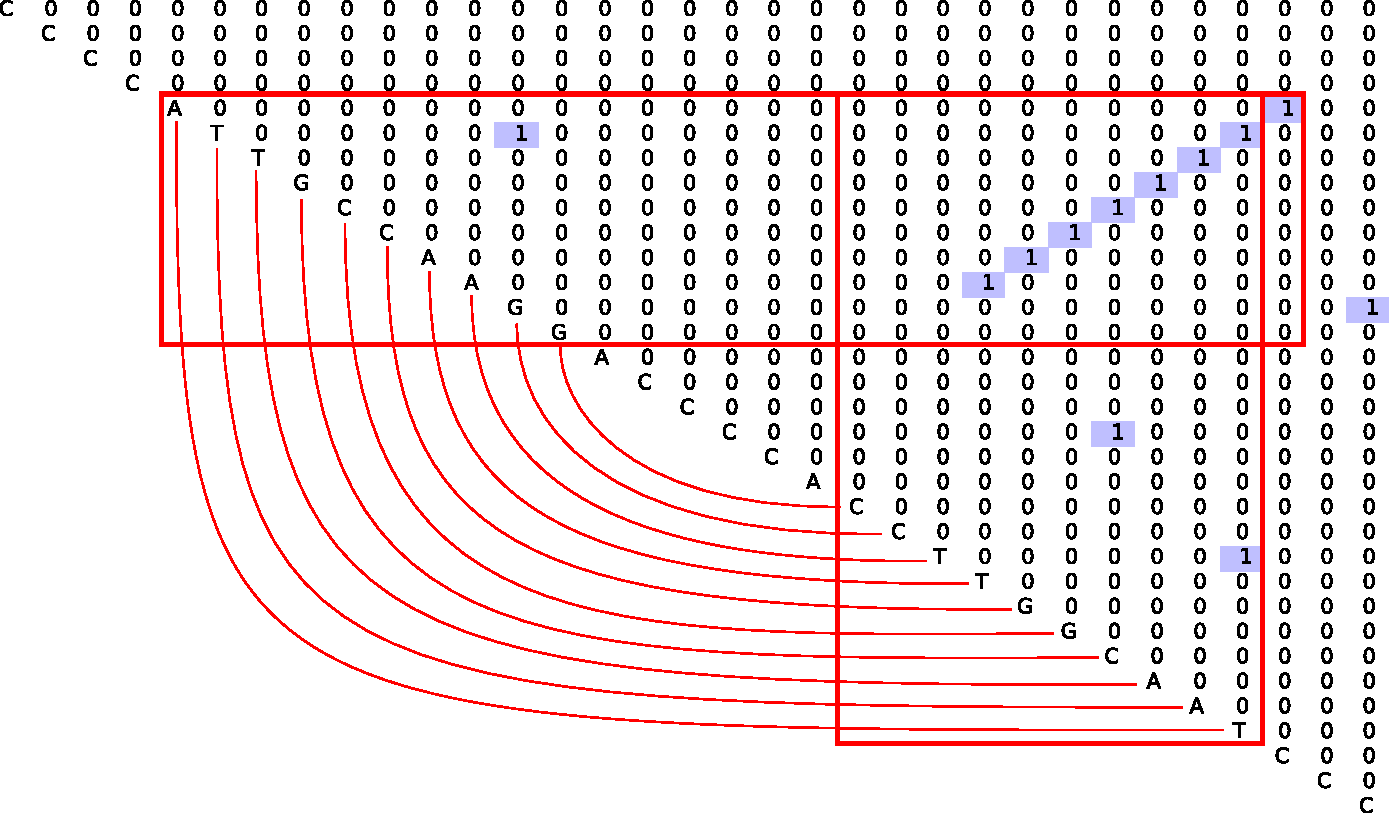
\includegraphics[width=0.8\textwidth]{figures/4.pdf}
\caption{Parsing result for sequence which should fold to
stem}
\label{fig:example}
\end{center}
\end{figure}

The parsing result in a form of matrix can be linearized, compressed into a byte or int vector, and be further handled by a dense neural network, as described in~\cite{grigorevcomposition}.
Unfortunately, linearization breaks data locality: a chain of $1$, which signifies a high stem, is local in a matrix, but is broken apart during its linearization.
We see it to be an argument to investigate the applicability of convolutional networks for parsing result handling as a boolean matrix can be converted to a black-white bitmap image.
In this paper we provide an empirical comparison of networks which handle vectors and images.

Another problem is a bad performance of the earlier solution.
Since the trained network handles parsing result, each input sequence should first be parsed.
Parsing is a very time-consuming step: context-free parsing has cubic complexity in terms of the input length.
Even if we use matrix-based parsing algorithm~\cite{Azimov:2018:CPQ:3210259.3210264} which utilizes GPGPU, performance is insufficient.
We believe it would be better to avoid the parsing step at the final stage of the solution.
In this work, we propose a way to solve this problem by building a network which handles raw sequences, not parsing results.

\section{The solution}
In this paper we improve the solution proposed in~\cite{grigorevcomposition}. We provide some ideas that are aimed to optimize its quality and performance and solve the problems that we faced during the experimental research.

First, we describe how to use convolutional network for parsing result processing. Parsing result is a boolean matrix and we utilize the artificial neural network to detect sufficient features and to find patterns in their appearance.
Therefore, we need to transform these boolean matrices to some data structure acceptable by the neural network.
Presently, we came up with two possible ways.

The first one is to drop out the nullary bottom left triangle, vectorize the top right triangle row by row and transform it into a byte vector.
This approach reduces the input size, but it requires all the input sequences to have equal length.
Thus we propose to either cut sequences to be of some predefined length or to pad them up with some blank symbols.
Vectorisation breaks data locality which makes learning harder: the network should restore back the relations broken during linearization.
This also means that the learning takes more time.

The second way is to represent the matrix as an image: the false bits of the matrix as white pixels and the true bits as black ones.
This approach makes it possible to process sequences of different lengths since the images are easily transformed to a specified size.
Data locality is also preserved: the information about relative positions of extracted basic features does not get lost which should improve learning.

The architecture of neural network that takes vectorized data as an input is described in~\cite{grigorevcomposition} and it consists of the long sequence of interchangeable dense and dropout layers with aggressive batch normalization. To handle images, we propose use a network which consists of a small number of convolutional layers, linearization, and dense network which has a similar architecture as for vectorized data.
In this paper we provide an evaluation on both data formats and compare the results.

Another improvement that we came up with concerns parsing elimination in the context of our solution. The idea is to create a model which can handle original sequences instead of the parsing matrices. For that, we propose to use two-staged learning: first, a network which solves a subtask is trained and then it is used as pretrained layers in the training of the resulting network.
In our solution we first train a neural network to handle parsing results which performs classification according to a problem at hands. We create two networks in order to compare different architectures: one of them handles vectorized parsing result, the other handles parsing result represented as a bitmap image. After that, we extend these neural networks by a number of input layers that take the initial nucleotide sequence as an input and convert it to the parsing result which is handled appropriately by the pretrained layers.

Figure~\ref{nn} represents the detailed description of these three neural networks architectures.
Here \textbf{\texttt{N1}} is a network which handles images, \textbf{\texttt{N2}} is a network which handles vectorized parsing results, and \textbf{\texttt{N0}} is an additional block which converts the input sequence into a set of features which can be handled by using \textbf{\texttt{N1}} or \textbf{\texttt{N2}}. So, firstly we train \textbf{\texttt{N1}} and \textbf{\texttt{N2}} on parsed data. After that, for vector-based network we combine the extension \textbf{\texttt{N0}} and the whole original sequence of layers and for image-based network we use the similar architecture, except we remove the convolutional layer from the extended model, thus, the first layer at the junction of the blocks corresponds to the linearized image.

\begin{figure}[h]
\begin{center}
\centering
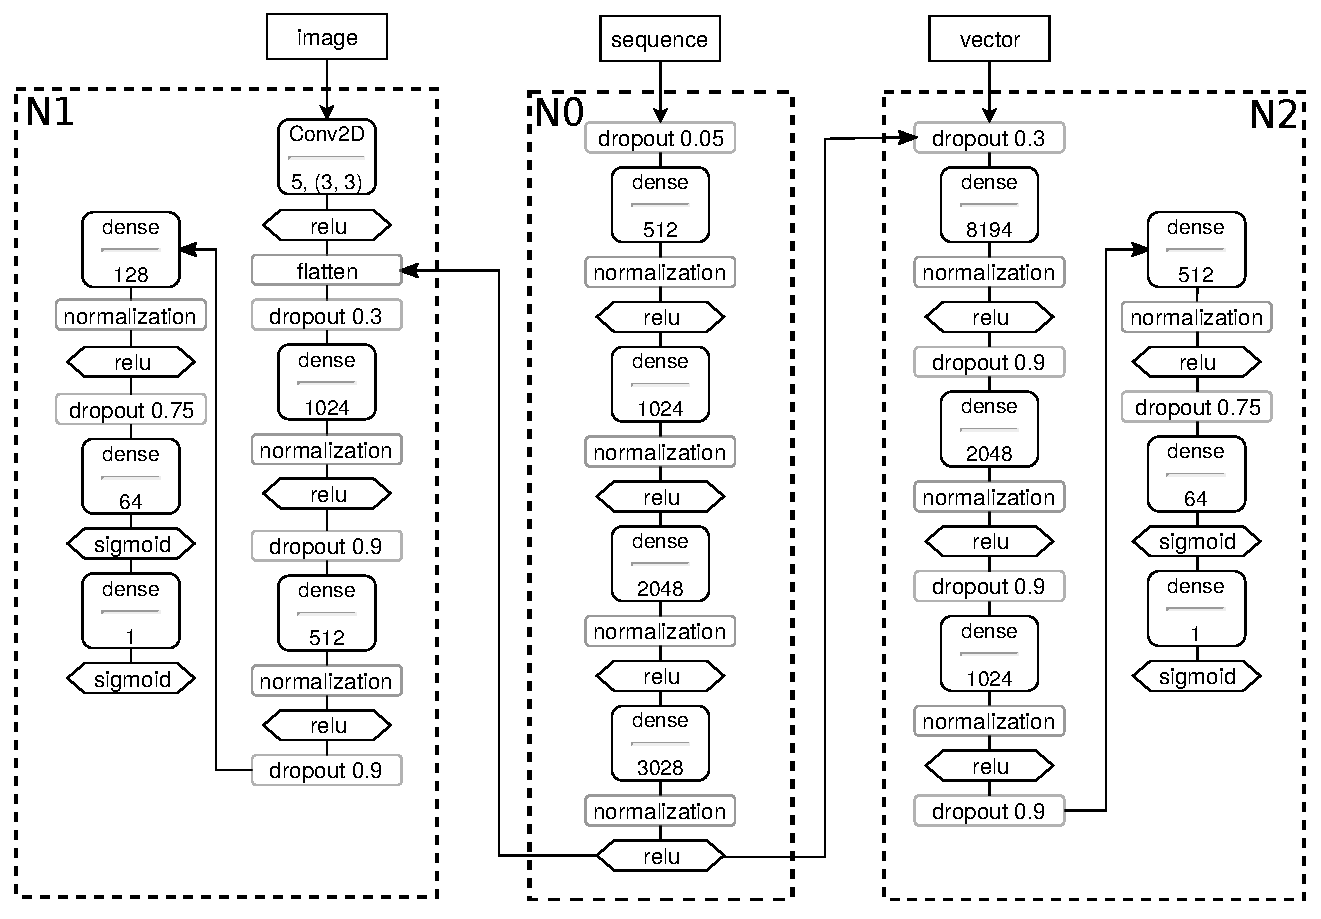
\includegraphics[width=12cm]{figures/nn_arch.pdf}
\caption{Neural networks architectures}
\label{nn}
\end{center}
\end{figure}

To sum up, we developed a technique to process parsing matrices as images by convolutional neural networks. Also we built a model that handles sequences and requires parsing only for training the network it is based on. This removes the parsing step from the usage of the trained model.

\section{Experiments}
We evaluated the proposed approach with the described above modifications on two tRNA sequences analysis tasks.
The first one was a classification of tRNA into two classes: eukaryotes and prokaryotes, while the second was a classification into four classes: archaea, bacteria, plants and fungi.
We took sequences from tRNA databases~\cite{trnadb1,trnadb2} for these experiments. We used parsing algorithm implemented by means of the YaccConstructor platform~\cite{yaccconstructor} and Keras library~\cite{keras} with Tensorflow framework~\cite{tensorflow} for neural networks training and testing. All models as well as parsing tool were run on GPU NVIDIA GeForce GTX 1070.

We selected the equal number of samples (single tRNA molecule sequences) for each class for both classification tasks.
Each sample was parsed w.r.t. the grammar $G_0$ and then both vectorized and transformed into an image.
After that, we trained two neural networks: first handles the representation of the parsing result as vectors, and the second~--- as images.
Finally, we trained the extended neural network.
It consists of a block which takes an initial tRNA sequence as an input and transforms it into the parsing result and the block of pretrained layers: either the vector- or the image-based model from the previous step. 

All extended neural networks were trained, validated (by hold-out validation) and tested on the same datasets as the corresponding base ones.
The trained models for two classes (EP) and for four classes (ABFP) classification tasks were estimated by using classical machine learning metrics: accuracy, precision and recall.

Accuracy metrics for each problem for the test datasets are presented in the table~\ref{acc}, where base model is a model which handles parsing result (image or vector respectively) and extended model handles tRNA sequences and extends the corresponding base model.

\begin{table}[h]
\centering
\caption{Base and extended models test results by accuracy metrics}
\begin{tabular}{|l||l|l||l|l|}
\hline
Classifier                                                               & \multicolumn{2}{l||}{EP}               & \multicolumn{2}{l|}{ABFP}           \\ \hline \hline
Approach                                                                 & Vector-based       & Image-based      & Vector-based      & Image-based     \\ \hline
\begin{tabular}[c]{@{}l@{}}Base model\\ accuracy\end{tabular}            & 94.1\%             & 96.2\%           & 86.7\%            & 93.3\%          \\ \hline
\begin{tabular}[c]{@{}l@{}}Extended model \\ accuracy\end{tabular}       & 97.5\%             & 97.8\%           & 96.2\%            & 95.7\%          \\ \hline
\begin{tabular}[c]{@{}l@{}}Total training \\ time\end{tabular}       & 30000s             & 4600s           & 31800s            & 3600s          \\ \hline
\begin{tabular}[c]{@{}l@{}}Samples for\\ train:valid:test\end{tabular} & \multicolumn{2}{l||}{\begin{tabular}[c]{@{}l@{}}20000:5000:10000\\ (57\%:14\%:29\%)\end{tabular}} & \multicolumn{2}{l|}{\begin{tabular}[c]{@{}l@{}}8000:1000:3000\\ (67\%:8\%:25\%)\end{tabular}} \\ \hline
\end{tabular}
\label{acc}
\end{table}


The estimations by precision and recall metrics for extended models for both classifiers on the same samples as in the  table~\ref{acc} are presented in the table~\ref{pe}.

\begin{table}[h]
\centering
\caption{Models test results by precision and recall metrics for each class}
\begin{tabular}{|l||l|l|l|l|l|}
\hline
\multirow{2}{*}{Classifier} & \multirow{2}{*}{Class} & \multicolumn{2}{l|}{Vector-based approach} & \multicolumn{2}{l|}{Image-based approach} \\ \cline{3-6} 
                            &                        & precision         & recall        & precision        & recall        \\ \hline \hline
\multirow{2}{*}{EP}         & prokaryotic            & 95.8\%            & 99.4\%        & 96.2\%           & 99.4\%        \\ \cline{2-6} 
                            & eukaryotic             & 99.4\%            & 95.6\%        & 99.4\%           & 99.5\%        \\ \hline \hline
\multirow{4}{*}{ABFP}       & archaeal               & 91.1\%            & 99.2\%        & 91.6\%           & 98.5\%        \\ \cline{2-6} 
                            & bacterial              & 96.6\%            & 95.1\%        & 95.2\%           & 95.5\%        \\ \cline{2-6} 
                            & fungi                  & 98.5\%            & 94.9\%        & 97.5\%           & 94.3\%        \\ \cline{2-6} 
                            & plant                  & 99.4\%            & 95.7\%        & 99.2\%           & 94.7\%        \\ \hline
\end{tabular}
\label{pe}
\end{table}

The results show that our approach is applicable to tRNA classification tasks and both vector- and image-based models can be used along with dense and convolutional layers in neural networks architectures.
While the differences in results for extended models are insignificant, for base models image-based network demonstrates slightly better results (see table~\ref{acc}).
We believe that the reason of this effect lays in a better locality of features in the image-based representation of parsing result: chain of $1$ which means a high stem is local in terms of picture, but is broken during linearization. 
Also we analysed the time spent on all the models training (table~\ref{acc}) and, although some of these numbers could probably be decreased by more detailed networks tuning, we can state that image-based networks learn much faster than vector-based ones.
Current model for images classification uses a single convolution layer.
Whether it is possible to utilize deep convolutional networks for secondary structure analysis in the discussed approach is a question for future research.

The idea of extended model that handles sequences instead of parsing result is proved to be applicable in practice and it demonstrates even higher quality than the original parsing-based model, as illustrated by table~\ref{acc}.
We can conclude that it is possible to use parsing only for network training without decreasing the network quality.

To demonstrate the advantage of this technique in practical use 
in comparison with the classical way when sequences should first be parsed we took 100 tRNA sequences from two classes: eukaryotes and prokaryotes and used all four of the trained models to predict their classes. While using base models each sequence was parsed, transformed to correspondent format (image or vector) and fed to the neural network. Extended networks run on original sequences, so the parsing step was skipped. We measured total time required to output predicted class for all the considered sequences in each case. In the table~\ref{time} the results are provided and it is clear that the time spent for parsing is crucial relatively to the total working time. So, the parsing eliminating modification significantly improves the performance of our solution.


\begin{table}[]
\centering
\caption{Time measurements for 100 sequences processing}
\begin{tabular}{|p{2cm}||p{2cm}|p{2cm}|p{2cm}|p{2cm}|}
\hline
\multirow{2}{*}{Step} & \multicolumn{2}{l|}{Vector based approach} & \multicolumn{2}{l|}{Image based approach} \\ \cline{2-5} 
 & \begin{tabular}[c]{@{}l@{}}Base \end{tabular} & \begin{tabular}[c]{@{}l@{}}Extended \end{tabular} & \begin{tabular}[c]{@{}l@{}}Base \end{tabular} & \begin{tabular}[c]{@{}l@{}}Extended \end{tabular} \\ \hline \hline
Parse & 307.6s & --- & 310.5s & --- \\ \hline
Load weights & 0.2s & 0.2s & 0.1s & 0.3s \\ \hline
Predict class & 0.2s & 0.2s & 0.2s & 0.3s \\ \hline
Total & 308.0s & 0.4s & 310.8s & 0.6s \\ \hline
\end{tabular}
\label{time}
\end{table}

\section{Conclusion}
We describe the modifications of the proposed approach for biological sequences analysis using the combination of formal grammars and neural networks.
We show that it is possible to handle parsing result which is represented as an image by using convolutional layers while processing it with a neural network, and it improves the quality of the solution.
Also, we provide a solution that removes the parsing step from the trained model use and allows to run models on the original RNA sequences.
As a result, the performance of the solution is significantly improved.
We demonstrate the applicability of the proposed modifications for real-world problems.
Source code and documentation are published at GitHub: \url{https://github.com/LuninaPolina/SecondaryStructureAnalyzer}.

We can provide several directions for future research.
First of all, it is necessary to investigate the applicability of the proposed approach for other sequences processing tasks such as 16s rRNA processing and chimeric sequences filtration.

Another possible application is a secondary structure prediction.
Is it possible to create a generative network which generates the most possible contact map for the given sequence?

The image-based model demonstrates higher quality.
We believe that it is caused by a better locality of features.
If so, it should be possible to create deep convolutional network for secondary structure analysis: further investigation is needed.

Finally, it is important to find a theoretical base for grammar tuning.
Is it possible to use theoretical results on secondary structure description by using formal grammar, such as~\cite{MQbioinformatics19} to find the optimal grammar for our approach?
%
% ---- Bibliography ----
%
% BibTeX users should specify bibliography style 'splncs04'.
% References will then be sorted and formatted in the correct style.
%
% \bibliographystyle{splncs04}
% \bibliography{mybibliography}
%
\begin{thebibliography}{14}

\bibitem{dowell2004evaluation}
Dowell, R.D., Eddy, S.R.: Evaluation of several lightweight stochastic context-free grammars for RNA secondary structure prediction. BMC bioinformatics \textbf{5}(1), 71 (2004)

\bibitem{knudsen1999rna}
Knudsen, B., Hein, J.: RNA secondary structure prediction using stochastic context-free grammars and evolutionary history. Bioinformatics (Oxford, England) \textbf{15}(6) 446--454 (1999)

\bibitem{EddyDurbin}
Durbin, R., Eddy, S.R., Krogh, A., Mitchison, G.: Biological sequence analysis: probabilistic models of proteins and nucleic acids. Cambridge university press (1998)

\bibitem{Infernal}
Nawrocki, E. P., Eddy, S. R.: Infernal 1.1: 100-fold faster RNA homology searches. Bioinformatics \textbf{29}(22) 2933--2935 (2013)

\bibitem{Humidor}
Sherman, D.: Humidor: Microbial community classification of the 16s gene by training cigar strings with convolutional neural networks. (2017)

\bibitem{ANN}
Higashi, S., Hungria, M., Brunetto, M.: Bacteria classification based on 16S ribosomal gene using artificial neural networks. In: Proceedings of the 8th WSEAS International Conference on Computational intelligence, man-machine systems and cybernetics. pp. 86--91. World Scientific and Engineering Academy and Society (2009)

\bibitem{grigorevcomposition}
Grigorev, S., Lunina, P.: The Composition of Dense Neural Networks and Formal Grammars for Secondary Structure Analysis. In:Proceedings of the 12th International Joint Conference on Biomedical Engineering Systems and Technologies - Volume 3: BIOINFORMATICS. pp. 234--241. SciTePress (2019)

\bibitem{MQbioinformatics19}
Quadrini, M., Merelli, E., Piergallini, R.: Loop Grammars to Identify RNA Structural Patterns. In: Proceedings of the 12th International Joint Conference on Biomedical Engineering Systems and Technologies - Volume 3: BIOINFORMATICS. pp 302--309. SciTePress (2019)

\bibitem{Azimov:2018:CPQ:3210259.3210264}
Azimov, R., Grigorev, S.: Context-free path querying by matrix multiplication. In: Proceedings of the 1st ACM SIGMOD Joint International Workshop on Graph Data Management Experiences \& Systems (GRADES) and Network Data Analytics (NDA). pp. 5:1--5:10. ACM(2018)


\bibitem{trnadb1}
Genomic tRNA Database, \url{http://gtrnadb.ucsc.edu/}. Last accessed 5 June 2019

\bibitem{trnadb2}
tRNADB-CE, \url{http://trna.ie.niigata-u.ac.jp/cgi-bin/trnadb/index.cgi}. Last accessed 5 June 2019

\bibitem{yaccconstructor}
YaccConstructor, \url{https://github.com/YaccConstructor}. Last accessed 12 Feb 2020

\bibitem{keras}
Keras, \url{https://keras.io}. Last accessed 12 Feb 2020

\bibitem{tensorflow}
TensorFlow, \url{https://www.tensorflow.org/}. Last accessed 12 Feb 2020

\iffalse
\bibitem{ref_article1}
Author, F.: Article title. Journal \textbf{2}(5), 99--110 (2016)

\bibitem{ref_lncs1}
Author, F., Author, S.: Title of a proceedings paper. In: Editor,
F., Editor, S. (eds.) CONFERENCE 2016, LNCS, vol. 9999, pp. 1--13.
Springer, Heidelberg (2016). \doi{10.10007/1234567890}

\bibitem{ref_book1}
Author, F., Author, S., Author, T.: Book title. 2nd edn. Publisher,
Location (1999)

\bibitem{ref_proc1}
Author, A.-B.: Contribution title. In: 9th International Proceedings
on Proceedings, pp. 1--2. Publisher, Location (2010)

\bibitem{ref_url1}
LNCS Homepage, \url{http://www.springer.com/lncs}. Last accessed 4
Oct 2017
\fi
\end{thebibliography}
\end{document}
